% arara: lualatex: {shell: yes}
% arara: biber 
% arara: lualatex: {shell: yes}
% arara: lualatex: {shell: yes}


\documentclass[english,xcolor={rgb,dvipsnames,table,usenames}]{beamer}

\mode<presentation> {

\usecolortheme{magpie}

}

\usepackage{cancel}
\usepackage{multirow}
\usepackage{graphicx}
\usepackage{booktabs}
%\usepackage[french]{babel}
\usepackage[utf8]{inputenc}
\usepackage[T1]{fontenc}
\usepackage{colortbl}
\usepackage{pgfplots}
\usepackage{array,multirow,makecell}
\usepackage{dsfont}
\usepackage{stmaryrd}
\usepackage{multicol}
\usepackage{changepage}
\usepackage{amsmath}
\usepackage{amssymb}
\usepackage{amsfonts}
\usepackage{bm}
% \usepackage{biblatex}
\usepackage[export]{adjustbox}
\usepackage{slashbox}
\usepackage{xcolor}
\usepackage{pict2e}
\usepackage{pifont}
\usepackage{eurosym}
%\usepackage{pst-all}
\usepackage{tikz}
\usetikzlibrary{arrows,intersections,positioning,shapes.arrows,decorations.markings,overlay-beamer-styles}
\usepackage{ulem}
\usepackage[customcolors]{hf-tikz}
%\usepackage{subcaption}
%\usepackage{pdfpages}
\usepackage{hyperref}
\usepackage{mdframed}
\usepackage{listings}
\usepackage{caption}
\usepackage{subcaption}
%\usepackage[backend=biber,safeinputenc,refsection=chapter]{biblatex}
\usepackage[backend=biber,bibencoding=utf8]{biblatex}
%\usepgfplotslibrary{external} 
%\tikzexternalize
\usepackage{animate}


\definecolor{links}{HTML}{2A1B81}
\hypersetup{colorlinks,linkcolor=,urlcolor=links}

\tikzset{style green/.style={
    set fill color=green!50!lime!60,
    set border color=white,
  },
  style cyan/.style={
    set fill color=cyan!90!blue!60,
    set border color=white,
  },
  style orange/.style={
    set fill color=orange!80!red!60,
    set border color=white,
  },
  hor/.style={
    above left offset={-0.15,0.31},
    below right offset={0.15,-0.125},
    #1
  },
  ver/.style={
    above left offset={-0.1,0.3},
    below right offset={0.15,-0.15},
    #1
  }
}

\newcommand{\tikzmark}[2][minimum width=6cm,minimum height=1.5cm]{
\tikz[remember picture, overlay]
\node[anchor=west,
inner sep=0pt,
outer sep=6pt,
xshift=-0.5em,
yshift=-3ex,
#1](#2){};
}

\newcommand{\norm}[1]{\left\lVert#1\right\rVert}

\addbibresource{biblioDisc.bib}


\newcommand{\cmark}{\ding{51}}
\newcommand{\xmark}{\ding{55}}

\setcellgapes{1pt}
\makegapedcells
\newcolumntype{R}[1]{>{\raggedleft\arraybackslash }b{#1}}
\newcolumntype{L}[1]{>{\raggedright\arraybackslash }b{#1}}
\newcolumntype{C}[1]{>{\centering\arraybackslash }b{#1}}

\DeclareMathOperator*{\argmin}{\arg\!\min}
\DeclareMathOperator*{\argmax}{\arg\!\max}

\newcommand{\xuparrow}[1]{%
  {\left\uparrow\vbox to #1{}\right.\kern-\nulldelimiterspace}
}

\tikzset{
  treenode/.style = {shape=rectangle, rounded corners,
                     draw, align=center,
                     top color=white, bottom color=blue!20},
  root/.style     = {treenode, font=\Large, bottom color=red!30},
  env/.style      = {treenode, font=\ttfamily\normalsize},
  dummy/.style    = {circle,draw}
}


% Allows the use of \toprule, \midrule and \bottomrule in tables

%----------------------------------------------------------------------------------------
%	TITLE PAGE
%----------------------------------------------------------------------------------------

\title[Prof. Assist. DIX]{Audition Prof. Assistant en Sciences des Données et Intelligence Artificielle}

\author{Adrien Ehrhardt}
\institute[CACF - Inria]
{

\normalsize

% \textit{aehrhardt@ca-cf.fr} % Your email address
}
\date{14/05/2019} % Date, can be changed to a custom date

\titlegraphic{%
    
\includegraphics[width=2.5cm]{inria.png}~%
    
\includegraphics[width=4cm]{logo.png}%
}

% \logo{%
%     
\includegraphics[width=1cm]{inria.jpg}~%
%     
\includegraphics[width=1.5cm]{logo.png}%
% }

\AtBeginSection[]{
  \begin{frame}
  \vfill
  \centering
  \begin{beamercolorbox}[sep=8pt,center,shadow=true,rounded=true]{title}
    \usebeamerfont{title}\insertsectionhead\par%
  \end{beamercolorbox}
  \vfill
  \end{frame}
}

\tikzset{
    myarrow/.style={
        draw,
        fill=orange,
        single arrow,
        minimum height=3.5ex,
        single arrow head extend=1ex
    }
}

 \tikzset{
    highlight on/.style={alt={#1{fill=red!80!black,color=red!80!black}{fill=gray!30!white,color=gray!30!white}}},
}


\tikzstyle{interrupt}=[
    postaction={
        decorate,
        decoration={markings,
                    mark= at position 0.5 
                          with
                          {
                            \fill[black] (-0.1,-0.3) rectangle (0.1,0.3);
                            \draw (-0.1,0.3) -- (-0.1,-0.3)
                                  (0.1,0.3) -- (0.1,-0.3);
                          }
                    }
                }
]


\addtobeamertemplate{navigation symbols}{}{%
    \usebeamerfont{footline}%
    \usebeamercolor[fg]{footline}%
    \hspace{1em}%
    \insertframenumber/\inserttotalframenumber
}

\lstset{language=R}

\newcommand{\appropto}{\mathrel{\vcenter{
  \offinterlineskip\halign{\hfil$##$\cr
    \propto\cr\noalign{\kern2pt}\sim\cr\noalign{\kern-2pt}}}}}

\newcommand\q{{\bm{q}}}
\newcommand\s{q}
\newcommand\Q{\mathcal{Q}}
\newcommand\ag{\bm{\alpha}}
\newcommand{\bth}{\boldsymbol{\theta}} 
\newcommand{\bc}{\boldsymbol{c}} 
\newcommand{\bx}{\boldsymbol{x}} 
\newcommand{\tx}{\textbf{x}}
\newcommand{\bs}{\boldsymbol{s}} 
\newcommand{\ts}{\textbf{s}}
\newcommand{\be}{\boldsymbol{e}} 
\newcommand{\te}{\textbf{e}}
\newcommand{\by}{\boldsymbol{y}} 
\newcommand{\ty}{\textbf{y}}

\def\mybar#1#2#3{%%
\begin{tabular}{@{}l@{}} {\scriptsize #1} \\ {\scriptsize #2} \\ {\scriptsize #3} \end{tabular} & \resizebox{.05#1\textwidth}{0.7cm}{\begin{tabular}{@{}l@{}}{\color{green}\rule[0pt]{#1bp}{10pt}} \\ {\color{orange}\rule[0pt]{#2bp}{10pt}} \\ {\color{red}\rule[0pt]{#3bp}{10pt}} \end{tabular}}}


\def\myobar#1#2#3{%%
\begin{tabular}{@{}l@{}} {\scriptsize #1} \\ {\scriptsize #2} \\ {\scriptsize #3} \end{tabular} & \resizebox{.05#2\textwidth}{0.7cm}{\begin{tabular}{@{}l@{}}{\color{orange}\rule[0pt]{#1bp}{10pt}} \\ {\color{green}\rule[0pt]{#2bp}{10pt}} \\ {\color{orange}\rule[0pt]{#3bp}{10pt}}\end{tabular}}}

\newcommand{\myGlobalTransformation}[2]
{
    \pgftransformcm{1}{0}{0.4}{0.5}{\pgfpoint{#1cm}{#2cm}}
}


\newcommand{\myGlobalTransformationbis}[2]
{
    \pgftransformcm{1}{0}{0.4}{0.3}{\pgfpoint{#1cm}{#2cm}}
}

\newcommand{\gridThreeD}[3]
{
    \begin{scope}
        \myGlobalTransformation{#1}{#2};
        \draw [#3,step=7cm] grid (7,7);
    \end{scope}
}

\tikzstyle myBG=[line width=3pt,opacity=1.0]

\newcommand{\drawLinewithBG}[2]
{
    \draw[white,myBG]  (#1) -- (#2);
    \draw[black,very thick] (#1) -- (#2);
}

\newcommand{\graphLinesHorizontal}
{
    \drawLinewithBG{1,1}{7,1};
    \drawLinewithBG{1,3}{7,3};
    \drawLinewithBG{1,5}{7,5};
    \drawLinewithBG{1,7}{7,7};
}

\newcommand{\graphLinesVertical}
{
    %swaps x and y coordinate (hence vertical lines):
    \pgftransformcm{0}{1}{1}{0}{\pgfpoint{0cm}{0cm}}
    \graphLinesHorizontal;
}

\newcommand{\graphThreeDnodes}[2]
{
    \begin{scope}
        \myGlobalTransformation{#1}{#2};
        \foreach \x in {1,3,5,7} {
            \foreach \y in {1,3,5,7} {
                \node at (\x,\y) [circle,fill=black,scale=0.3] {};
                %this way circle of nodes will not be transformed
            }
        }
    \end{scope}
}

%\setbeamercovered{transparent} 
\setbeamercolor{itemize item}{fg=red}
\setbeamercolor{itemize subitem}{fg=red}
\setbeamertemplate{itemize/enumerate body begin}{\footnotesize}
\setbeamertemplate{itemize/enumerate subbody begin}{\footnotesize}

\begin{document}

\pgfmathdeclarefunction{gauss}{2}{\pgfmathparse{1/(#2*sqrt(2*pi))*exp(-((x-#1)^2)/(2*#2^2))}}

\frame[plain]{\titlepage}



\begin{frame}
\frametitle{Table of Contents}
\tableofcontents[hideallsubsections]
\end{frame}

%\def\beamertemplatetransparentcoveredmedium{\setbeamercovered{transparent=50}}
%\beamertemplatetransparentcoveredmedium


\section{Short Bio}

\begin{frame}
\frametitle{\secname}

\begin{tikzpicture}[xscale=0.9]
\draw[line width=1mm,-latex,red!20] (-0.2,0) -- (10+0.2,0);
\foreach \X [evaluate=\X as \Y using int(\X-2010),count=\Z] in {2010,2012,2015,2019}
{
\draw[highlight on=<\Z>] ({\Y-0.2},-0.5) -- ({\Y+0.2},-0.5) -- (\Y,-0.1) -- cycle;
\node[anchor=south,highlight on=<\Z>,fill=black,rotate=45,anchor=south
west,inner sep=0pt] at (\Y,0.2) {\X};
}
\end{tikzpicture}
\begin{itemize}
\item<1-> 2010: BAC S \& start of MPSI / MPI preparatory classes in Strasbourg;
\item<2-> 2012: \'Ecole Centrale de Lille;
\begin{itemize}
\item 2014: B.Sc. (Licence 3) of Mathematics at Université de Lille;
\item 2014: Research project in integer programming;
\item 2014: Internship at Eiffage Group $\approx$ penalized regression;
\item 2015: ``Décision et Analyse de Données'' specialization + apprenticeship at BNP Paribas as a Quant.\ Analyst.
\end{itemize}
\item<3-> 2015: Crédit Agricole Consumer Finance
\begin{itemize}
\item 11/2015: Data Scientist position (permanent contract);
\item 04/2016: Official start of the CIFRE funding;
\end{itemize}
\item<4-> 2019: 
\begin{itemize}
\item 04/2019: Official end of the CIFRE funding;
\item Mid-07/2019: Defense;
\item 09/2019: Part-time Ass.\ Prof.\ + (current position + telework | position in the ``Groupe de Recherches Opérationnelles'').
\end{itemize}
\end{itemize}


\end{frame}




\section{Research}

\subsection{the industrial setting}

\begin{frame}
\frametitle{\secname : \subsecname}

\only<1-6>{
\begin{table}
\centering
\begin{tiny}
\hspace*{-0.7cm}\begin{tabular}{p{1.7cm}|p{1.1cm}|p{1cm}|p{1.4cm}|p{1.5cm}||p{0.6cm}|p{1cm}}
\textcolor <4,6> {OliveGreen} {\textbf<4,6>{Job}} & \only<1-3>{Home} & \only<1-3>{Time in job} & \textcolor <4,6> {OliveGreen} {\textbf<4,6>{Family status}} & \textcolor <4,5> {OliveGreen} {\textbf<4,5>{Wages}} & \uncover<8->{\textcolor{OliveGreen}{\textbf{Score}}} & Repayment \\
\hline
\textcolor <4,6> {OliveGreen} {\textbf<4,6>{\only<1-5>{Craftsman} \only<6->{?+Low-qualified}}} & \only<1-3>{Owner} & \only<1-3>{20} & \textcolor <4,6> {OliveGreen} {\textbf<4,6>{\only<1-5>{Widower}  \only<6>{?+Alone}}} & \textcolor <4-5> {OliveGreen} {\textbf<4-5>{\only<1-4>{2000} \only<5->{]1500;2000]}}} & \uncover<8->{\textcolor{OliveGreen}{\textbf{225}}} & 0  \\
\textcolor <4,6> {OliveGreen} {\textbf<4,6>{\only<1-5>{?} \only<6->{?+Low-qualified}}} & \only<1-3>{Renter} & \only<1-3>{10} & \textcolor <4,6> {OliveGreen} {\textbf<4,6>{\only<1-5>{Common-law}  \only<6>{Union}}} & \textcolor <4-5> {OliveGreen} {\textbf<4>{\only<1-4>{1700} \only<5->{]1500;2000]}}} & \uncover<8->{\textcolor{OliveGreen}{\textbf{190}}} & 1  \\
\textcolor <4,6> {OliveGreen} {\textbf<4,6>{\only<1-5>{Licensed professional} \only<6->{High-qualified}}} & \only<1-3>{Starter} & \only<1-3>{5} & \textcolor <4,6> {OliveGreen} {\textbf<4,6>{\only<1-5>{Divorced} \only<6>{?+Alone}}} & \textcolor <4-5> {OliveGreen} {\textbf<4>{\only<1-4>{4000} \only<5->{]2000;$\infty$[}}} & \uncover<8->{\textcolor{OliveGreen}{\textbf{218}}} & 0  \\
\textcolor <4,6> {OliveGreen} {\textbf<4,6>{\only<1-5>{Executive} \only<6->{High-qualified}}} & \only<1-3>{By work} & \only<1-3>{8} & \textcolor <4,6> {OliveGreen} {\textbf<4,6>{\only<1-5>{Single} \only<6>{?+Alone}}} & \textcolor <4-5> {OliveGreen} {\textbf<4>{\only<1-4>{2700} \only<5->{]2000;$\infty$[}}} & \uncover<8->{\textcolor{OliveGreen}{\textbf{202}}} & 1  \\
\textcolor <3> {OliveGreen} {\textbf<3>{\only<1-2>{{Office employee}} \only<3->{\cancel{Office employee}}}} &  \textcolor <3> {OliveGreen} {\textbf<3>{\only<1-2>{Renter} \only<3->{\cancel{Renter}}}} & \textcolor <3> {OliveGreen} {\textbf<3>{\only<1-2>{12} \only<3->{\cancel{12}}}} & \textcolor <3> {OliveGreen} {\textbf<3>{\only<1-2>{Married} \only<3->{\cancel{Married}}}} & \textcolor <3> {OliveGreen} {\textbf<3>{\only<1-2>{1400} \only<3->{\cancel{1400}}}} & \uncover<8->{\textcolor{OliveGreen}{\textbf{NA}}} & NA  \\
\textcolor <3> {OliveGreen} {\textbf<3>{\only<1-2>{Worker} \only<3->{\cancel{Worker}}}} & \textcolor <3> {OliveGreen} {\textbf<3>{\only<1-2>{By family} \only<3->{\cancel{By family}}}} & \textcolor <3> {OliveGreen} {\textbf<3>{\only<1-2>{2} \only<3->{\cancel{2}}}} & \textcolor <3> {OliveGreen} {\textbf<3>{\only<1-2>{?} \only<3->{\cancel{?}}}} & \textcolor <3> {OliveGreen} {\textbf<3>{\only<1-2>{1200} \only<3->{\cancel{1200}}}} & \uncover<8->{{\textbf{NA}}} & NA  \\
\end{tabular}
\end{tiny}
\caption{\label{tab:exemple} Dataset with outliers and missing values.} 
\end{table}
}

\only<7>{
\begin{table}
\centering
\begin{tiny}
\hspace*{-0.7cm}\begin{tabular}{p{2cm}|p{1.1cm}|p{1cm}|p{2.4cm}||p{0.6cm}|p{1cm}}
\textcolor <4,6> {OliveGreen} {\textbf<4,6>{Job}} & \only<2-3>{Home} & \only<2-3>{Time in job} & \textcolor <7> {OliveGreen} {\textbf<7>{Family status x Wages}} & \uncover<8->{\textcolor{OliveGreen}{\textbf{Score}}} & Repayment \\
\hline
\textcolor <4,6> {OliveGreen} {\textbf<4,6>{\only<2-5>{Craftsman} \only<6->{?+Low-qualified}}} & \only<2-3>{Owner} & \only<2-3>{20} & \textcolor <7> {OliveGreen} {\textbf<6>{?+Alone x ]1500;2000]}} & \uncover<8->{\textcolor{OliveGreen}{\textbf{225}}} & 0  \\
\textcolor <4,6> {OliveGreen} {\textbf<4,6>{\only<2-5>{?} \only<6->{?+Low-qualified}}} & \only<2-3>{Renter} & \only<2-3>{10} & \textcolor <7> {OliveGreen} {\textbf<7>{Union x ]1500;2000]}} & \uncover<8->{\textcolor{OliveGreen}{\textbf{190}}} & 1  \\
\textcolor <4,6> {OliveGreen} {\textbf<4,6>{\only<2-5>{Licensed professional} \only<6->{High-qualified}}} & \only<2-3>{Starter} & \only<2-3>{5} & \textcolor <7> {OliveGreen} {\textbf<7>{?+Alone x ]2000;$\infty$[}} & \uncover<8->{\textcolor{OliveGreen}{\textbf{218}}} & 0  \\
\textcolor <4,6> {OliveGreen} {\textbf<4,6>{\only<2-5>{Executive} \only<6->{High-qualified}}} & \only<2-3>{By work} & \only<2-3>{8} & \textcolor <7> {OliveGreen} {\textbf<7>{?+Alone x ]2000;$\infty$[}} & \uncover<8->{\textcolor{OliveGreen}{\textbf{202}}} & 1  \\
\textcolor <3> {OliveGreen} {\textbf<3>{\only<1-2>{{Office employee}} \only<3->{\cancel{Office employee}}}} &  \textcolor <3> {OliveGreen} {\textbf<3>{\only<1-2>{Renter} \only<3->{\cancel{Renter}}}} & \textcolor <3> {OliveGreen} {\textbf<3>{\only<1-2>{12} \only<3->{\cancel{12}}}} & \textcolor <3> {OliveGreen} {\textbf<3>{\only<1-2>{Married} \only<3->{\cancel{Married}}}} \textcolor <3> {OliveGreen} {\textbf<3>{\only<1-2>{1400} \only<3->{\cancel{1400}}}} & \uncover<8->{{\textbf{NA}}} & NA  \\
\textcolor <3> {OliveGreen} {\textbf<3>{\only<1-2>{Worker} \only<3->{\cancel{Worker}}}} & \textcolor <3> {OliveGreen} {\textbf<3>{\only<1-2>{By family} \only<3->{\cancel{By family}}}} & \textcolor <3> {OliveGreen} {\textbf<3>{\only<1-2>{2} \only<3->{\cancel{2}}}} & \textcolor <3> {OliveGreen} {\textbf<3>{\only<1-2>{?} \only<3->{\cancel{?}}}} \textcolor <3> {OliveGreen} {\textbf<3>{\only<1-2>{1200} \only<3->{\cancel{1200}}}} & \uncover<8->{{\textbf{NA}}} & NA  \\
\end{tabular}
\end{tiny}
\caption{\label{tab:exemple} Dataset with outliers and missing values.}
\end{table}
}

\only<8->{
\begin{table}
\centering
\begin{tiny}
\hspace*{-0.7cm}\begin{tabular}{p{2cm}|p{1.1cm}|p{1cm}|p{2.4cm}||p{0.6cm}|p{1cm}}
\textcolor <4,6> {OliveGreen} {\textbf<4,6>{Job}} & \only<2-3>{Home} & \only<2-3>{Time in job} & \textcolor <7> {OliveGreen} {\textbf<7>{Family status x Wages}} & \uncover<9->{\textcolor{OliveGreen}{\textbf{Score}}} & Repayment \\
\hline
\textcolor <4,6> {OliveGreen} {\textbf<4,6>{\only<2-5>{Craftsman} \only<6->{?+Low-qualified}}} & \only<2-3>{Owner} & \only<2-3>{20} & \textcolor <7> {OliveGreen} {\textbf<6>{?+Alone x ]1500;2000]}} & \uncover<9->{\textcolor{OliveGreen}{\textbf{225}}} & 0  \\
\textcolor <4,6> {OliveGreen} {\textbf<4,6>{\only<2-5>{?} \only<6->{?+Low-qualified}}} & \only<2-3>{Renter} & \only<2-3>{10} & \textcolor <7> {OliveGreen} {\textbf<7>{Union x ]1500;2000]}} & \uncover<9->{\textcolor{OliveGreen}{\textbf{190}}} & 1  \\
\hline
\textcolor <4,6> {OliveGreen} {\textbf<4,6>{\only<2-5>{Licensed professional} \only<6->{High-qualified}}} & \only<2-3>{Starter} & \only<2-3>{5} & \textcolor <7> {OliveGreen} {\textbf<7>{?+Alone x ]2000;$\infty$[}} & \uncover<9->{\textcolor{OliveGreen}{\textbf{218}}} & 0  \\
\textcolor <4,6> {OliveGreen} {\textbf<4,6>{\only<2-5>{Executive} \only<6->{High-qualified}}} & \only<2-3>{By work} & \only<2-3>{8} & \textcolor <7> {OliveGreen} {\textbf<7>{?+Alone x ]2000;$\infty$[}} & \uncover<9->{\textcolor{OliveGreen}{\textbf{202}}} & 1  \\
\textcolor <3> {OliveGreen} {\textbf<3>{\only<1-2>{{Office employee}} \only<3->{\cancel{Office employee}}}} &  \textcolor <3> {OliveGreen} {\textbf<3>{\only<1-2>{Renter} \only<3->{\cancel{Renter}}}} & \textcolor <3> {OliveGreen} {\textbf<3>{\only<1-2>{12} \only<3->{\cancel{12}}}} & \textcolor <3> {OliveGreen} {\textbf<3>{\only<1-2>{Married} \only<3->{\cancel{Married}}}} \textcolor <3> {OliveGreen} {\textbf<3>{\only<1-2>{1400} \only<3->{\cancel{1400}}}} & \uncover<9->{{\textbf{NA}}} & NA  \\
\textcolor <3> {OliveGreen} {\textbf<3>{\only<1-2>{Worker} \only<3->{\cancel{Worker}}}} & \textcolor <3> {OliveGreen} {\textbf<3>{\only<1-2>{By family} \only<3->{\cancel{By family}}}} & \textcolor <3> {OliveGreen} {\textbf<3>{\only<1-2>{2} \only<3->{\cancel{2}}}} & \textcolor <3> {OliveGreen} {\textbf<3>{\only<1-2>{?} \only<3->{\cancel{?}}}} \textcolor <3> {OliveGreen} {\textbf<3>{\only<1-2>{1200} \only<3->{\cancel{1200}}}} & \uncover<9->{{\textbf{NA}}} & NA  \\
\end{tabular}
\end{tiny}
\caption{\label{tab:exemple} Dataset with outliers and missing values.}
\end{table}
}
\vspace{-0.5cm}
\uncover<2->{
\begin{enumerate}
\item \textcolor <3> {OliveGreen} {\textbf<3>{Discarding rejected applicants}}
\item \textcolor <4> {OliveGreen} {\textbf<4>{Feature selection}}
\item \textcolor <5> {OliveGreen} {\textbf<5>{Discretization}} / \textcolor <6> {OliveGreen} {\textbf<6>{grouping}}
\item \textcolor <7> {OliveGreen} {\textbf<7>{Interaction screening}}
\item \textcolor <8> {OliveGreen} {\textbf<8>{Segmentation}}
\item \textcolor <9> {OliveGreen} {\textbf<9>{Logistic regression fitting}}
\end{enumerate}
}

\end{frame}

\setbeamertemplate{itemize/enumerate body begin}{\normalsize}
\setbeamertemplate{itemize/enumerate subbody begin}{\normalsize}


\subsection{four main topics tackled in the PhD}

\begin{frame}
\frametitle{\secname : \subsecname}

\normalsize

\begin{enumerate}
\item<1-> ``Reject Inference''

2 conferences; 1 ongoing paper; 1 \textsf{R} package.

\medskip

\item<2-> ``Quantization'': discretization + grouping.

1 conference; 1 submitted preprint; 2 packages.

\medskip

\item<3-> Pairwise interactions.

1 ongoing paper (w.\ another estimation technique for quantization).

\medskip

\item<4-> Segmentation
\end{enumerate}

\end{frame}


\subsection{reject inference}

%\begin{frame}
%\frametitle{\secname : \subsecname}
%
%\textbf{Problem setting:}
%
%\begin{figure}[ht]
%\begin{minipage}[b]{0.45\linewidth}
%\center 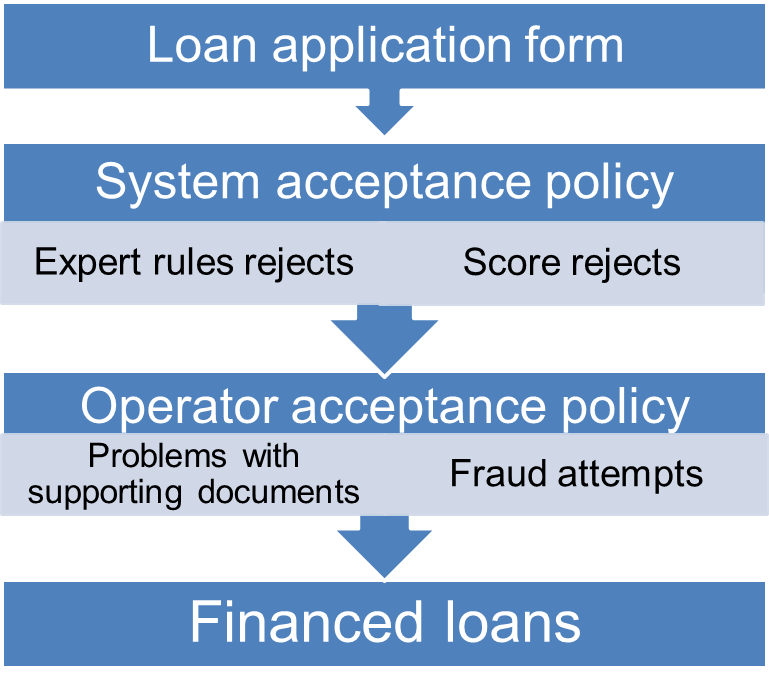
\includegraphics[width=5cm]{schema.png}
%\caption{Simplified Acceptance mechanism in~Crédit Agricole Consumer Finance.}
%\label{fig:figure1}
%
%\end{minipage}%
%\hfil \begin{minipage}[b]{0.5\linewidth}
%
%\center 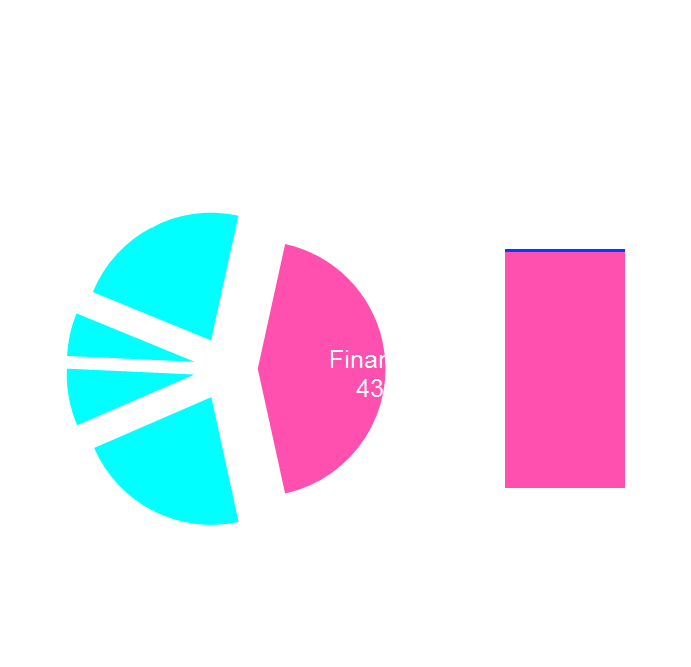
\includegraphics[width=5cm]{camembert_invert.png}
%\caption{Final decisions on the applications.}
%
%\end{minipage}
%\end{figure}
%
%\end{frame}




\begin{frame}
\frametitle{\secname : \subsecname}

\footnotesize

We have the following available data:

\setbeamercolor{normal text}{fg=black}
\usebeamercolor[fg]{normal text}


\[ \begin{array}{c}
\tikzmarkin[hor=style green]{el11} \bm{y}^{\text{f}} \tikzmarkend{el11}\\
\\
\\
\tikzmarkin[hor=style orange]{el12} \bm{y}^{\text{nf}} \tikzmarkend{el12}\end{array}
\left( \begin{array}{c}
\tikzmarkin[hor=style green]{e4} y_1 \\
\vdots \\
y_n \tikzmarkend{e4} \\ 
\tikzmarkin[hor=style orange]{e3} \text{NA} \\
\vdots \\
\text{NA} \tikzmarkend{e3} \end{array} \right) \hspace{1.5cm} \begin{array}{c}
\tikzmarkin[hor=style green]{el02} \bm{x}^{\text{f}} \tikzmarkend{el02}\\
\\
\\
\tikzmarkin[hor=style orange]{el-12} \bm{x}^{\text{nf}} \tikzmarkend{el-12} \end{array}
\left( \begin{array}{ccc}
%\rowcolor{red!20}
\tikzmarkin[hor=style green]{e1} \; \; x_1^1 & \cdots & x_1^d  \\
 \vdots & \vdots & \vdots  \\
 x_n^1 & \cdots & x_n^d \tikzmarkend{e1} \\
\tikzmarkin[hor=style orange]{e2} \; \; x_{n+1}^1 & \cdots & x_{n+1}^d  \\
 \vdots & \vdots & \vdots \\
 x_{n+m}^1 & \cdots & x_{n+m}^d \tikzmarkend{e2} \end{array} \right)\]
 
  
\setbeamercolor{normal text}{fg=white}
\usebeamercolor[fg]{normal text}


We usually fit a logistic regression using the observed data:
\[ \hat{\theta}^{\text{f}} = \argmin \text{CRIT}(\theta ; \bm{x}^{\text{f}}, \bm{y}^{\text{f}}). \]
We wish we had:
\[ \hat{\theta} = \argmin \text{CRIT}(\theta ; \bm{x}, \bm{y}). \]
Which cannot be computed since we lack $\bm{y}^{\text{nf}}$.

What's the relation between $\hat{\theta}^{\text{f}}$ and $\hat{\theta}$?
\end{frame}




\begin{frame}
\frametitle{\secname : \subsecname}

\footnotesize

For logistic regression, \textit{ad hoc} were proposed:
\setbeamercolor{normal text}{fg=black}
\usebeamercolor[fg]{normal text}
 \[ \begin{array}{c}
\tikzmarkin[hor=style green]{l1} \bm{y}^{\text{f}} \tikzmarkend{l1}\\
\\
\\
\tikzmarkin[hor=style green]{l2} \bm{y}^{\text{nf}} \tikzmarkend{l2} \end{array}
\left( \begin{array}{c}
\tikzmarkin[hor=style green]{l3} y_1 \\
\vdots \\
 y_n \\ 
 \hat{y}_{n+1} \\
\vdots \\
\hat{y}_{n+m} \tikzmarkend{l3}\end{array} \right) \begin{array}{c}
\tikzmarkin[hor=style green]{el0} \bm{x}^{\text{f}} \tikzmarkend{el0} \\
\\
\\
\tikzmarkin[hor=style green]{el-1} \bm{x}^{\text{nf}} \tikzmarkend{el-1} \end{array}
\left( \begin{array}{ccc}
%\rowcolor{red!20}
\tikzmarkin[hor=style green]{el1} \; \; x_1^1 & \cdots & x_1^d  \\
 \vdots & \vdots & \vdots \\
 x_n^1 & \cdots & x_n^d \\
 x_{n+1}^1 & \cdots & x_{n+1}^d  \\
 \vdots & \vdots & \vdots \\
 x_{n+m}^1 & \cdots & x_{n+m}^d \tikzmarkend{el1} \end{array} \right)\]

 
\setbeamercolor{normal text}{fg=white}
\usebeamercolor[fg]{normal text}


$\Rightarrow$ formalize and justify these methods, if possible.

%\textbf{Long story short}, methods:
%\begin{itemize}
%\item are useless ($\hat{\theta}^{\text{méthode}} = \hat{\theta}^{\text{f}}$) ;
%\item require additional ``hypotheses'':
%\begin{itemize}
%\item additional estimation = bias + variance ;
%\item cannot be compared to a ``gold standard'' car $\cancel{\bm{y}^\text{nf}}$;
%\end{itemize}
%\item are ``worse'' than $\hat{\theta}^{\text{f}}$.
%\end{itemize}

\end{frame}





\subsection{quantization}

{
\setbeamercolor{background canvas}{bg=white}
\begin{frame}
\frametitle{\secname : \subsecname}

\begin{figure}[!ht]
\begin{animateinline}[poster=first, controls=all, palindrome, autopause, autoresume, width=\textwidth, height=6cm]{3}
\multiframe{99}{i=2+1}{\input{R_CODE_FIGURES/disc_plot\i.tex}}%
\end{animateinline}
%\caption{\label{fig:anim_sinus} Animation of logistic regression fits on data generated by a sinus with a number of discretization steps in the \textit{equal-length} algorithm ranging from 2 to 100.}
\end{figure}

\end{frame}
}


\begin{frame}
\frametitle{\secname : \subsecname}

\textbf{Problem setting:}

``Constrained'' representation learning:
\[ (\q^\star,\bth^\star) = \argmin_{\textcolor{red}{q \in \mathcal{Q}},\bth \in \Theta} \text{CRIT}(\hat{\bth}_{q}). \]

\uncover<2->{
\textbf{Resolution:}

Relaxation of the search for the number of cutpoints and their location as a continuous problem.

\begin{center}
\begin{tikzpicture}[scale=0.3]
\draw[->,line width=0.1cm] (-5,0)--(24,0) node[right]{$x_j$};

\node [red,circle, fill] at (4,0) {};
\node [red,circle, fill] at (12,0) {};

\node at (4,-1.5) {$c_{j,1}$};
\node at (12,-1.5) {$c_{j,2}$};

\node at (-1,1) {$(1,0,0)$};
\node at (8,1) {$(0,1,0)$};
\node at (19,1) {$(0,0,1)$};

\end{tikzpicture}
\end{center}
}
\end{frame}


\begin{frame}
\frametitle{\secname : \subsecname}

\begin{tikzpicture}[scale=0.9]
\begin{axis}[
  no markers, domain=-1.5:2, samples=100,
  axis lines*=left,
  every axis y label/.style={at=(current axis.left of origin), anchor=north west},
  height=3cm, width=11cm,
  xtick=\empty, ytick=\empty,
  enlargelimits=false, clip=false,
  x label style={at={(axis description cs:0.5,-0.1)},anchor=north},
  y label style={at={(axis description cs:-0.1,.5)},rotate=90,anchor=south},
  xlabel={$x_j$},
  ylabel={$\s_{\hat{\ag}_{j,1}}(x_j)$}
  ]
    
  \addplot [very thick,white] {gauss(-1.8,0.6)};
\addplot+[mark=none,thick,red] coordinates {(-0.7,0) (-0.7,0.6)};
\addplot+[mark=none,thick,red] coordinates {(1,0) (1,0.6)};
\node at (axis cs:-1.1,0.4) {$\hat{\s}_{j,1}(x_j)=1$};
\node at (axis cs:0,0.4) {$\hat{\s}_{j,1}(x_j)=0$};
\node at (axis cs:1.5,0.4) {$\hat{\s}_{j,1}(x_j)=0$};
\node at (axis cs:-0.7,-0.15) {$\hat{c}_{j,1}$};
\node at (axis cs:1,-0.15) {$\hat{c}_{j,2}$};

\end{axis}
\end{tikzpicture}

\begin{tikzpicture}[scale=0.9]
\begin{axis}[
  no markers, domain=-1.5:2, samples=100,
  axis lines*=left,
  every axis y label/.style={at=(current axis.left of origin), anchor=north west},
  height=3cm, width=11cm,
  xtick=\empty, ytick=\empty,
  enlargelimits=false, clip=false,
  x label style={at={(axis description cs:0.5,-0.1)},anchor=north},
  y label style={at={(axis description cs:-0.1,.5)},rotate=90,anchor=south},
  xlabel={$x_j$},
  ylabel={$\s_{\hat{\ag}_{j,2}}(x_j)$}
  ]
    
  \addplot [very thick,white] {gauss(0,0.6)};
\addplot+[mark=none, thick,red] coordinates {(-0.7,0) (-0.7,0.6)};
\addplot+[mark=none, thick,red] coordinates {(1,0) (1,0.6)};
\node at (axis cs:-1.1,0.4) {$\hat{\s}_{j,2}(x_j)=0$};
\node at (axis cs:0,0.4) {$\hat{\s}_{j,2}(x_j)=1$};
\node at (axis cs:1.5,0.4) {$\hat{\s}_{j,2}(x_j)=0$};
\node at (axis cs:-0.7,-0.15) {$\hat{c}_{j,1}$};
\node at (axis cs:1,-0.15) {$\hat{c}_{j,2}$};

\end{axis}

\end{tikzpicture}

\begin{tikzpicture}[scale=0.9]
\begin{axis}[
  no markers, domain=-1.5:2, samples=100,
  axis lines*=left,
  every axis y label/.style={at=(current axis.left of origin), anchor=north west},
  height=3cm, width=11cm,
  xtick=\empty, ytick=\empty,
  enlargelimits=false, clip=false,
  x label style={at={(axis description cs:0.5,-0.1)},anchor=north},
  y label style={at={(axis description cs:-0.1,.5)},rotate=90,anchor=south},
  xlabel={$x_j$},
  ylabel={$\s_{\hat{\ag}_{j,3}}(x_j)$}
  ]
    
  \addplot [very thick,white] {gauss(2,0.6)};

\addplot+[mark=none, thick,red] coordinates {(-0.7,0) (-0.7,0.6)};
\addplot+[mark=none, thick,red] coordinates {(1,0) (1,0.6)};

\node at (axis cs:-1.1,0.4) {$\hat{\s}_{j,3}(x_j)=0$};
\node at (axis cs:0,0.4) {$\hat{\s}_{j,3}(x_j)=0$};
\node at (axis cs:1.5,0.4) {$\hat{\s}_{j,3}(x_j)=1$};
\node at (axis cs:-0.7,-0.15) {$\hat{c}_{j,1}$};
\node at (axis cs:1,-0.15) {$\hat{c}_{j,2}$};

\end{axis}
\end{tikzpicture}
\end{frame}

%\begin{frame}
%\frametitle{\secname : \subsecname}
%
%This new model can be estimated either:
%\begin{itemize}
%\item<1> By a straightforward neural network that acts as a computation graph;
%
%\medskip
%
%Works well, pretty fast since it relies on standard DL libraries.
%\item<2> By considering the quantized features as latent features, and resort to stochastic optimization, \textit{e.g.}\ an SEM-algorithm.
%
%\medskip
%
%Integrates well with our proposal for the ``interactions'' problem; explores well quantization with less than a user-defined number of cuts / groups.
%\end{itemize}
%
%\end{frame}


\subsection{interactions}

\begin{frame}
\frametitle{\secname : \subsecname}

\textbf{Problem setting:}

%Upper triangular matrix with $\delta_{k,\ell} = 1 $ if $k < \ell$ and features p and q ``interact'' in the logistic regression.
\[ \text{logit}(p_{\bm{\theta}}(1|\bm{x})) = \theta_0 + x ' \theta + \sum_{1\leq k < \ell \leq d} \delta_{k,\ell} x_k ' \theta_{k,\ell} x_{\ell} \]
\uncover<2->{
%Imagine for now that the quantization $\q(\bm{x})$ is fixed. The criterion becomes:
\begin{align*}
(\bm{\theta}^\star,\bm{\delta}^\star) & = \argmax_{\bm{\theta},\textcolor{red}{\bm{\delta} \in \{0,1\}^\frac{d(d-1)}{2}}} \text{CRIT}(\hat{\theta}_{\delta})
\end{align*}
}

\uncover<3->{
Analogous to previous problem: $2^{\frac{d(d-1)}{2}}$ models.
}

\uncover<4->{
$\delta$ is latent and hard to optimize over: use a stochastic algorithm!
}

\end{frame}


\subsection{logistic regression trees}

\begin{frame}
\frametitle{\secname : \subsecname}

\textbf{Problem setting:}

\tikzstyle{level 1}=[level distance=1.5cm, sibling distance=9cm]
\tikzstyle{level 2}=[level distance=1.5cm, sibling distance=4.5cm]
\tikzstyle{level 3}=[level distance=2cm, sibling distance=3.5cm]


\resizebox{\linewidth}{!}{\begin{tikzpicture}
  [
    sibling distance        = 15em,
    level distance          = 5em,
    edge from parent/.style = {draw, -latex},
    every node/.style       = {font=\footnotesize},
    sloped
  ]
  \node [root] {\textcolor{black}{Clients}}
    child { node [dummy] {}
      child { node [dummy] {}
        child { node [env] {\textcolor{black}{$p_{\theta_1}(y|\bm{q}_{\{1\}}(\bm{x}_{\{1\}})$}}
          edge from parent node [below] {\textcolor{white}{Renters}} }
        child { node [env] {\textcolor{black}{$p_{\theta_2}(y|\bm{q}_{\{2\}}(\bm{x}_{\{2\}}))$}}
          edge from parent node [above] {\textcolor{white}{Workers}} }
        child { node [env] {\textcolor{black}{$p_{\theta_3}(y|\bm{q}_{\{3\}}(\bm{x}_{\{3\}}))$}}
                edge from parent node [above] {\textcolor{white}{Others}} }
        edge from parent node [above] {\textcolor{white}{Revolving}} }
      child { node [env] {\textcolor{black}{$p_{\theta_4}(y|\bm{q}_{\{4\}}(\bm{x}_{\{4\}}))$}}
              edge from parent node [above, align=center]
                {\textcolor{white}{Standard}} }
              edge from parent node [above] {\textcolor{white}{Appliances}} }
    child { node [dummy] {}
      child { node [dummy] {}
        child { node [env] {\textcolor{black}{$p_{\theta_5}(y|\bm{q}_{\{5\}}(\bm{x}_{\{5\}}))$}}
          edge from parent node [above] {\textcolor{white}{Leasing}} }
        child { node [env] {\textcolor{black}{$p_{\theta_6}(y|\bm{q}_{\{6\}}(\bm{x}_{\{6\}}))$}}
                edge from parent node [above] {\textcolor{white}{Standard}} }
        edge from parent node [above] {\textcolor{white}{Fiat}} }
      child { node [env] {\textcolor{black}{$p_{\theta_7}(y|\bm{q}_{\{7\}}(\bm{x}_{\{7\}}))$}}
              edge from parent node [above, align=center]
                {\textcolor{white}{Kawasaki}} }
              edge from parent node [above] {\textcolor{white}{Cars}} };
\end{tikzpicture}}


\end{frame}




\renewcommand{\footnotesize}{\tiny}

\begin{frame}
\frametitle{\secname : \subsecname}

\textbf{Current methodology:} unsupervised generative approaches such as PCA.

\bigskip

\textbf{State-Of-The-Art:}
LOTUS~\footfullcite{chan2004lotus} / LMT~\footfullcite{landwehr2005logistic} / MOB~\footfullcite{zeileis2008model}.

\bigskip

\uncover<2->{
\textbf{Proposed method:} smooth stochastic relaxation similar to the quantization problem.

\bigskip

\textbf{Results:}
Better than SOTA on simulated data.

Works well on real data where SOTA methods are intractable.
}
\end{frame}




\subsection{high dimensional unstructured data}

\begin{frame}
\frametitle{Bonus: \subsecname}

The banking industry is in a \textit{Big Data} era: gotta catch'em all!

\begin{enumerate}
\item Navigation data on Sofinco's website.

\item Transactional data (credit cards).

\end{enumerate}

\bigskip

How to use these ``dynamic'' features, stored on evolving Hadoop clusters, in traditional, parametric models such as logistic regression alongside  ``classical'' features, stored in relational databases?

\medskip

First few ideas: supervised generative clustering techniques, \textit{e.g.}\ functional PCA.

\end{frame}





\section{Teaching}

\subsection{past experience}

\begin{frame}[allowframebreaks]
\frametitle{\secname : \subsecname}

\begin{block}{DUT STID $1^{\text{st}}$ year - Université de Lille}

\textbf{Programmation statistique} - \textsf{R}

Aim: give an overview of data ingestion, data types, standard libraries and graphs, notebooks and basic statistics.
\end{block}

\begin{block}{GIS3 - Polytech' Lille}

\textbf{Statistique inférentielle} - \textsf{R}

Aim: rephrase an industrial problem with toy data into statistical tests, restitution as reports.

\medskip

\textbf{Régression linéaire} - \textsf{R}

Aim: perform linear regression (univariate then multivariate regression) and goodness-of-fit tests.
\end{block}

\pagebreak

\begin{block}{GIS4 - Polytech' Lille}

\textbf{Projet statistique} - \textsf{R}

Aim: perform an end-to-end analysis of a toy dataset (classification or clustering), structure it into a report and a presentation.
\end{block}

\begin{block}{Semaine d'\'Etudes Mathématiques-Entreprises}

Aim: provide PhD students with industry experience; proposed subject: profit estimation.
\end{block}

\begin{block}{G3 - Centrale Lille}

\textbf{Projet Impact} - Python

Aim: perform a ``real-life'' project in partnership with a company; proposed subject: quantization + interactions.

\end{block}

\end{frame}



\subsection{possible contribution}

\begin{frame}
\frametitle{\secname : \subsecname}

\begin{enumerate}
\item<1-> Courses in the Bachelor program

\medskip

$\approx$ similar level to what I've taught so far \textit{e.g.}\ CSE 101, 102, 204, Computer Science projects, which could benefit from my 
``industrial'' toolkit (R, Python, git, Docker) and potential projects with real datasets.

\bigskip

\item<2-> Data Science track of the 3A / M1 Herbrand

\medskip

In particular INF554, MAP573, MAP566 which are close to the day-to-day activities of a Data Scientist: pipeline, preprocessing, supervised learning, visualization, \dots

\end{enumerate}


\end{frame}




\begin{frame}

\Huge
Thank you!

\end{frame}




\begin{frame}
\frametitle{Publications}
\begin{scriptsize}

\fullcite{rjs}

\fullcite{jds}

\fullcite{jrss}

\fullcite{Rpackagescoring}

\fullcite{artDisc}

\fullcite{ds3}

\fullcite{compstat}

\fullcite{seminaireMED}

\fullcite{ehrhardt2019feature}

\end{scriptsize}
\end{frame}


\end{document}


